\section{Динамика движения материальной точки по окружности}
%Сив260
\AddProb С какой начальной скоростью $v_0$ должен вылететь снаряд из
орудия в горизонтальном направлении, чтобы двигаться вокруг Земли, не падая на нее? Каким ускорением будет обладать снаряд при этом (Радиус Земли $R = 6,4 \cdot 10^3$ км).
%Сив273
\AddProb Самолет делает «мертвую петлю» радиуса $R = 100$ м и движется по ней со скоростью $v = 280$ км/ч. С какой силой тело летчика массой в 80 кг будет давить на сиденье самолета в верхней и нижней точках петли?

%Сив264
\begin{wrapfigure}[11]{R}{3cm}
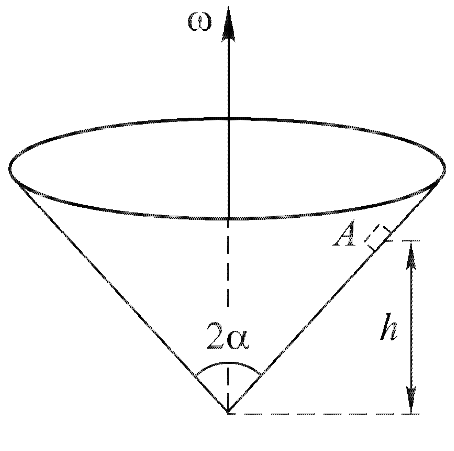
\includegraphics[width=0.3\textwidth]{Conus.png}
\caption{}
\label{Conus}
\end{wrapfigure}
\AddProb На внутренней поверхности конической воронки с углом $2\alpha$ при вершине (рис. \ref{Conus}) на высоте $h$ от вершины находится малое тело. Коэффициент трения между телом и поверхностью воронки равен $\mu$. Найти минимальную угловую скорость вращения конуса вокруг вертикальной оси, при которой тело будет неподвижно в воронке.
%Сив265
\AddProb Велосипедист при повороте по кругу радиуса $R$ наклоняется внутрь закругления так, что угол между плоскостью велосипеда и землей равен $\alpha$. Найти скорость $v$ велосипедиста.

%Сив285
\begin{wrapfigure}[10]{r}{2cm}
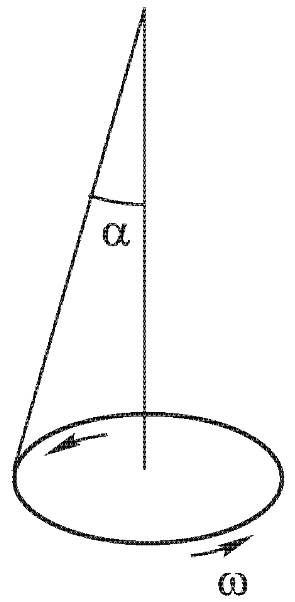
\includegraphics[width=0.2\textwidth]{RotationRing.png}
\caption{}
\label{RotationRing}
\end{wrapfigure}
\AddProb Металлическое кольцо, подвешенное на нити к оси центробежной машины, как указано на рис. \ref{RotationRing}, равномерно вращается с угловой скоростью $\omega$. Нить составляет
угол $\alpha$ с осью. Найти расстояние от центра кольца до оси вращения.

%Сив283
\begin{wrapfigure}[5]{r}{2cm}
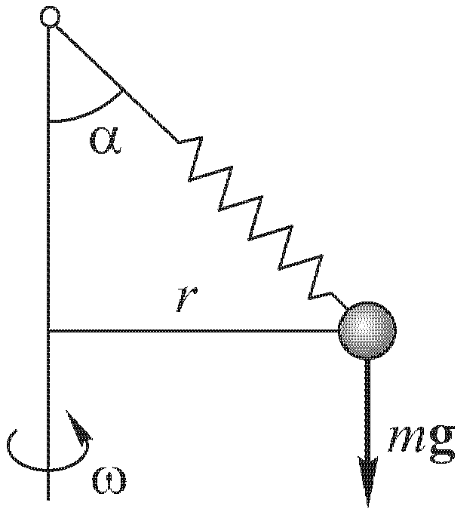
\includegraphics[width=0.2\textwidth]{CentrafugalMashine.png}
\caption{}
\label{CentrafugalMashine}
\end{wrapfigure}
\begin{wrapfigure}[9]{r}{3cm}
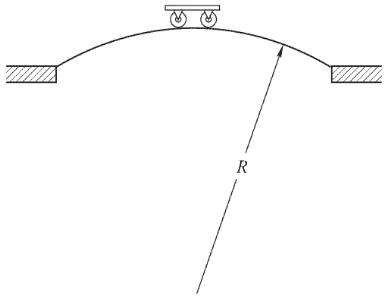
\includegraphics[width=0.3\textwidth]{Bridge.png}
\caption{}
\label{Bridge}
\end{wrapfigure}
\AddProb Шарик массы $m$ подвешен на идеальной пружине жесткости $	k$ и начальной длины $l$ над центром платформы центробежной
машины (рис. \ref{CentrafugalMashine}). Затем шарик начинает вращаться вместе с машиной с угловой скоростью $\omega$. Какой
угол $\alpha$ образует при этом пружина с вертикалью?

%Сив257
\AddProb Найти силу $F$, с которой тележка массы $m$, движущаяся со скоростью $v$, давит на мост в одном из следующих случаев: 1) горизонтальный мост; 2) выпуклый мост (рис. \ref{Bridge}); 3) вогнутый мост. (Для случаев 2) и 3) силу $F$ определить для наивысшей и наинизшей точек моста).

%Сив258
\begin{wrapfigure}[6]{r}{3cm}
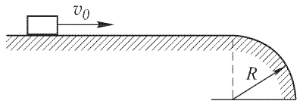
\includegraphics[width=0.3\textwidth]{Rounding.png}
\caption{}
\label{Rounding}
\end{wrapfigure}
\AddProb Тело движется прямолинейно с постоянной скоростью $v$ по
горизонтальной поверхности стола, которая имеет закругленный край
с постоянным радиусом закругления, равным $R$ (рис. \ref{Rounding}). Каково должно быть минимальное значение скорости $v_0$, чтобы тело, падая со стола, не касалось закругления?

%Сив262
\begin{wrapfigure}[9]{r}{3cm}
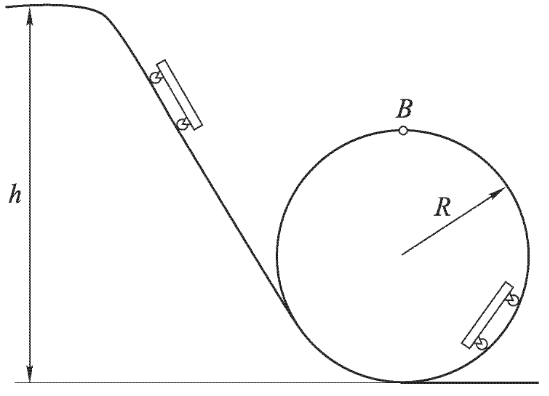
\includegraphics[width=0.3\textwidth]{DeathLoop.png}
\caption{}
\label{DeathLoop}
\end{wrapfigure}
\AddProb Тележка массы $m$ скатывается без трения по изогнутым
рельсам, имеющим форму, изображенную на рис. \ref{DeathLoop}. 1) С какой минимальной высоты $h$ должна скатиться тележка для того, чтобы она не покинула рельсов по всей их длине? 2) Какие силы действуют на тележку в наивысшей точке $В$ петли? 3) Каково будет движение тележки, если она скатывается с высоты, меньшей $h$? При решении задачи считать колеса тележки малого размера и малой массы и их вращательного движения не рассматривать.

\begin{wrapfigure}[9]{r}{1,5cm}
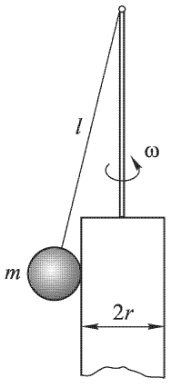
\includegraphics[width=0.15\textwidth]{CentrafugalMashine2.png}
\caption{}
\label{CentrafugalMashine2}
\end{wrapfigure}
%Сив263
\AddProb Каков должен быть минимальный коэффициент трения скольжения к между шинами автомобиля и асфальтом, чтобы автомобиль мог пройти закругление с радиусом $R = 200$ м при скорости $v = 100$ км/ч?
%Сив267
\AddProb Шарик радиуса $R$ висит на нити длины $l$ и касается вертикального цилиндра радиуса $r$, установленного на оси центробежной машины (рис. \ref{CentrafugalMashine2}). При какой угловой скорости и вращения центробежной машины шарик перестанет давить на стенку цилиндра?
%Сив269
\AddProb Шофер, едущий на автомобиле по горизонтальной площади в тумане, внезапно заметил недалеко впереди себя стену, перпендикулярную к направлению движения. Что выгоднее: затормозить или повернуть в сторону, чтобы предотвратить аварию?
%Сив272 
\AddProb При выполнении самолетом «мертвой петли», осуществленной
впервые русским летчиком П. Н. Нестеровым, сила, действующая на
крылья самолета, изменяется по сравнению с их нагрузкой при горизонтальном полете. Пусть самолет Нестерова массой в 3/4 т делает «мертвую петлю» радиуса $R = 235$ м и движется по ней со скоростью 120 км/ч. Найти максимальное значение нагрузки на крылья самолета. Указать, в каком месте траектории эта нагрузка будет максимальной.

%Сив276
\begin{wrapfigure}[9]{r}{3cm}
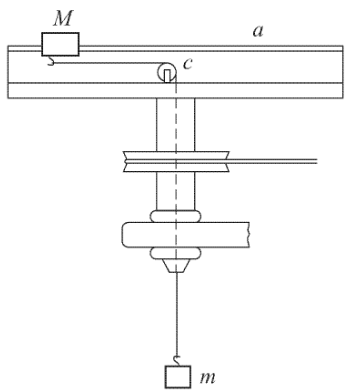
\includegraphics[width=0.3\textwidth]{CentrafugalMashine3.png}
\caption{}
\label{CentrafugalMashine3}
\end{wrapfigure}
\AddProb Груз массы $M$ может скользить без трения по стержню $a$,
укрепленному перпендикулярно к оси вращающейся центробежной машины (рис. \ref{CentrafugalMashine3}). Ось машины вертикальна, и сквозь нее проходит нить, на которой висит груз массы $m$; нить перекинута через блок с и другой ее конец прикреплен к грузу массы $M$. Найти положение груза массы $M$ на стержне $a$ когда центробежная машина вращается с угловой скоростью $\omega$.
\clearpage